% !TeX root = surprises.tex


\chapter{Konstruktion eines regelmäßigen Heptadekagons}\label{c.heptadecagon}

%%%%%%%%%%%%%%%%%%%%%%%%%%%%%%%%%%%%%%%%%%%%%%%%%%%%%%%%%%%%%%%

Die einzigen regelmäßigen Polygone, die die Griechen mit Lineal und Zirkel konstruieren konnten, waren das Dreieck, das Quadrat, das Fünfeck und das regelmäßige Polygon mit $15$ Seiten. Bei einem regelmäßigen Vieleck mit $n$ Seiten kann ein Vieleck mit $2n$ Seiten konstruiert werden, indem das Vieleck mit einem Kreis umschrieben und der zentrale Winkel halbiert wird (Abb.~\ref{f.hept-double}). Weitere Fortschritte wurden erst 1796 erzielt, als Carl Friedrich Gauß eines Morgens, kurz vor seinem 19. Geburtstag, erwachte und durch ``konzentriertes Denken'' herausfand, wie man ein regelmäßiges \emph{heptadecagon}, ein regelmäßiges Polygon mit $17$ Seiten konstruieren kann. Diese Leistung inspirierte ihn dazu, Mathematiker zu werden.

In Abschnitt~\ref{s.hept-regular} wird die Beziehung zwischen der Seite eines in einen Kreis eingeschriebenen Polygons und dem zentralen Winkel, den es einschließt, erörtert. Abschnitt~\ref{s.fundamental} gibt ohne Beweis den Fundamentalsatz der Algebra an. Abschnitt~\ref{s.roots} stellt die \emph{roots of unity} vor, die Wurzeln des Polynoms $x^n-1$, die im Mittelpunkt des Gaußschen Beweises stehen. Die Abschnitte~\ref{s.gauss} und~\ref{s.derivation} stellen den Beweis von Gauß vor, der auf Symmetrien der Wurzeln von Polynomen beruht. Gauß leitete eine Formel ab, die beweist, dass das Heptadeck konstruierbar ist, aber eine geometrische Konstruktion wurde fast ein Jahrhundert lang nicht gegeben. Abschnitt~\ref{s.construction} enthält eine elegante Konstruktion von James J. Callagy. Abschnitt~\ref{s.hept-pentagon} zeigt, wie Konstruktionen eines regelmäßigen Fünfecks sowohl aus der Geometrie als auch aus der Trigonometrie abgeleitet werden können.

Ein Teil des Materials ist einfacher, wenn es mit komplexen Zahlen dargestellt wird. Dieses Material ist in Kästen untergebracht, die übersprungen werden können.
\begin{figure}[t]
\begin{center}
\begin{tikzpicture}[scale=.4]
\coordinate (O) at (0,0);
\vertex{O};
\foreach \x/\name/\n/\po in {0/a/A/right,1/b/B/above,2/c/C/left,3/d/D/below left,4/e/E/below right} {
  \coordinate (\name) at ($(O)+(\x*72+18:3cm)$);
}
\draw (a) -- (b) -- (c) -- (d) -- (e) -- (a);
\node[draw,circle through=(a)] at (O) {};
\draw (d) -- (O) -- (e);
\draw [very thick,dotted] (O) -- (-90:3) -- (e) -- (-90:3) -- (d);
\end{tikzpicture}
\end{center}
\caption{Konstruktion eines regelmäßigen Polynoms mit $10$ Seiten aus einem regelmäßigen Fünfeck}\label{f.hept-double}
\end{figure}

\section{Konstruktion von regelmäßigen Polygonen}\label{s.hept-regular}

Die Konstruktion des regelmäßigen Heptadecks führte zum Gauß-Wantzel-Theorem, das besagt, dass ein regelmäßiges Polygon mit $n$ Seiten nur dann mit Lineal und Zirkel konstruiert werden kann, wenn $n$ das Produkt aus einer Potenz von $2$ und null oder mehr \emph{distinct} ist. Fermat-Zahlen{Fermat-Zahlen} $2^{2^k}+1$, die Primzahlen sind. Die bekannten Fermat-Primzahlen sind:
\[
F_0=3,\quad F_1=5,\quad F_2=17,\quad F_3=257,\quad F_4=65537\,.
\]
Ein regelmäßiges Polygon mit $257$ Seiten wurde von Magnus Georg Paucker in $1822$ und von Friedrich Julius Richelot $1832$ konstruiert. In $1894$ behauptete Johann Gustav Hermes, ein regelmäßiges Polygon mit $65537$ Seiten konstruiert zu haben.

\begin{figure}[b]
\begin{center}
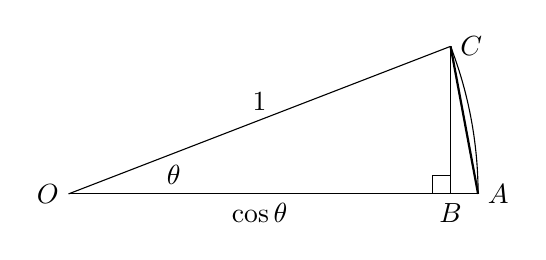
\begin{tikzpicture}[scale=1.3]
\coordinate (O) at (0,0) node[left] {$O$} node[above right,xshift=32pt] {$\theta$};
\coordinate (A) at (4,0);
\node[right] at (A) {$A$};
\draw (O) -- (A);
\draw (A) arc(0:21.12:4);
\coordinate (C) at (21.12:4cm);
\draw (O) -- node[above] {$1$} (C);
\node[right] at (C) {$C$};
\draw (C) -- (C |- A) coordinate (B);
\node[below] at (B) {$B$};
\draw[rotate=90] (B) rectangle +(5pt,5pt);
\draw[thick] (A) -- (C);
\path (O) -- node[below] {$\cos \theta$} (B); 
\end{tikzpicture}
\end{center}
\caption{Kosinus des zentralen Winkels eines regelmäßigen Polygons}\label{f.hept-central1}
\end{figure}

Um ein regelmäßiges Polygon zu konstruieren, reicht es aus, ein Liniensegment der Länge $\cos \theta$ zu konstruieren, wobei $\theta$ der zentrale Winkel ist, der von einer Sehne eingeschlossen wird, die eine in einen Einheitskreis eingeschriebene Seite des Polygons ist. Konstruieren Sie für die Strecke $\overline{OB}=\cos\theta$ eine Senkrechte bei $B$ und bezeichnen Sie ihren Schnittpunkt mit dem Einheitskreis mit $C$. Dann:
\begin{eqnarray*}
\cos \theta&=&\displaystyle\frac{\overline{OB}}{\overline{OC}}=\overline{OB}\\
\theta &=& \cos^{-1} (\overline{OB})\,.
\end{eqnarray*}
Die Sehne $\overline{AC}$ ist eine Seite des regelmäßigen Vielecks (Abb.~\ref{f.hept-central1}).

Ausgehend von einem Liniensegment der Länge $1$ sind die Längen konstruierbar, die sich aus Liniensegmenten bekannter Länge mit Hilfe der Operationen $\{+,-,\times,/,\surd\}$ gewinnen lassen (Sect.~\ref{s.trisect-constructible}). Gauß zeigte, dass $\cos(360^\circ/17)$, der Kosinus des Zentralwinkels eines Heptadecks, konstruierbar ist, da er nur durch diese Operationen ausgedrückt werden kann:
\begin{eqnarray*}
\cos\left(\frac{360^\circ}{17}\right) &=& 
-\frac{1}{16}+\frac{1}{16}\sqrt{17} + 
     \frac{1}{16}\sqrt{34-2\sqrt{17}}
    + \\
    &&
     \frac{1}{8}\sqrt{
     17+3\sqrt{17} - 
     \sqrt{34-2\sqrt{17}}
   -2
     \sqrt{34+2\sqrt{17}}
   }\,.
\end{eqnarray*}

\section{Der Fundamentalsatz der Algebra}\label{s.fundamental}

Das folgende Theorem wird ohne Beweis verwendet.

\begin{theorem}\label{thm.fundamental} Jedes Polynom vom Grad $n$ hat genau $n$ Wurzeln.
\end{theorem}

Die Aussage des Satzes wurde vereinfacht, da wir nur wissen müssen, dass $n$ Wurzeln \emph{existieren}.

\smallskip

\begin{advanced}
\textbf{Der Fundamentalsatz der Algebra} besagt, dass jedes nicht konstante Polynom vom Grad $n$ in einer einzigen Variablen mit \emph{komplexen} Koeffizienten genau $n$ \emph{komplexe} Wurzeln hat. 
Wenn es mehrere Wurzeln mit demselben Wert gibt, werden sie alle gezählt: $x^2-4x+4=(x-2)(x-2)$ hat zwei Wurzeln, die beide gleich $2$ sind.
Das Polynom $x^2+1$ mit ganzzahligen Koeffizienten hat zwei komplexe Wurzeln $\pm\sqrt{-1}$.
Obwohl es sich um endliche algebraische Gebilde handelt - Polynome vom Grad $n$ mit $n$ Wurzeln -, braucht man zum Beweis des Satzes Methoden der Analysis, meist der komplexen Analysis.
\end{advanced}

\section{Die Wurzeln der Einheit}\label{s.roots}

Nach dem Fundamentalsatz der Algebra (Thm.~\ref{thm.fundamental}) hat das Polynom $x^{n}-1$ $n$ Wurzeln für jede ganze Zahl $n> 1$. Eine Wurzel ist $x=1$, also gibt es $n-1$ weitere Wurzeln. Bezeichnen Sie eine dieser Wurzeln mit $r$. Da $r^{n}=1$ ist, heißt sie \emph{$n$-te Wurzel der Einheit}. Was ist mit $r^2$?
\[
(r^{2})^n=(r^{n})^2=1^2=1\,.
\]
Daraus folgt, dass die $n$-Zahlen:
\[
1, r, r^2, \ldots, r^{n-2}, r^{n-1}
\]
sind $n$-te Wurzeln der Einheit.

\begin{advanced}
Sei $r=\cos \left(\frac{2\pi}{n}\right) + i\sin \left(\frac{2\pi}{n}\right)$.
Nach der Formel von de Moivre:
\[
\left[\cos \left(\frac{2\pi}{n}\right) + i\sin  \left(\frac{2\pi}{n}\right)\right]^{n}=
\cos \left(\frac{2 n\pi}{n}\right) + i\sin  \left(\frac{2 n\pi}{n}\right)= 1\,.
\]
\end{advanced}
\begin{theorem}
Sei $n$ eine Primzahl und $r$ eine $n$-te Wurzel der Einheit. Dann:
\[
\{1,r,r^2,\ldots,r^{n-2},r^{n-1}\}
\]
sind verschieden, also sind sie \emph{all} die $n$-ten Wurzeln der Einheit.
\end{theorem}

\begin{proof}
Angenommen, die Potenzen sind nicht verschieden, so dass $r^i=r^j$ für einige $0\leq i<j\leq n-1$. Dann ist $r^j/r^i=r^{j-i}=1$, so dass es mindestens eine positive ganze Zahl $i'$ kleiner als $n$ gibt, für die $r^{i'}=1$ gilt. Sei $m$ die kleinste solche positive ganze Zahl. Durch den Divisionsalgorithmus für ganze Zahlen $n=ml+k$ für einige $0<l<n$ und $0\leq k<m$. Von:
\[
1=r^n=r^{ml+k}=(r^m)^l\cdot r^k=1^l\cdot r^k=r^k\,,
\]
haben wir $0\leq k<m$ und $r^k=1$. Da $m$ als die kleinste solche positive ganze Zahl definiert wurde, ist $k=0$ und $n=ml$ nicht prim.
\end{proof}

\begin{theorem} Seien $\{a_1,a_2,\ldots,a_{n-1},a_n\}$ die Wurzeln eines Polynoms $n$-ten Grades $f(x)$. Dann:
\begin{align}\label{eq.viete}
f(x) =(x-a_1) (x-a_2)\cdots (x-a_{n-1})(x-a_n)\,.
\end{align}
\end{theorem}

\begin{proof}
Ist $a_i$ eine Wurzel von $f(x)$, so ist per Definition $f(a_i)=0$:
\begin{eqnarray*}
f(a_i)&=&(a_i-a_1) (a_i-a_2)\cdots (a_i-a_{n-1})(a_i-a_n)\\
&=&\cdots (a_i-a_i) \cdots =0\,.
\end{eqnarray*}
Daher ist $f(x)=(x-a_i)g_i(x)$ für einige $g_i(x)$ und durch Induktion gilt dies für alle Wurzeln.
\end{proof}

Aus Gl.~\ref{eq.viete} ist leicht zu erkennen, dass der Koeffizient von $x^{n-1}$ ist:
\[
-(a_1+a_2+\cdots+a_{n-1}+a_n)\,.
\]
Da der Koeffizient von $x^{n-1}$ in $x^n-1$ für $n\geq 2$ Null ist, haben wir:
\begin{eqnarray*}
-(1+r+r^2+\cdots + r^{n-2}+r^{n-1})&=&0\\
r+r^2+\cdots + r^{n-2}+r^{n-1}&=&-1\,.
\end{eqnarray*}
Für das Heptadecagon ist dies:
\begin{multline}
r+r^2+r^3+r^4+r^5+r^6+r^7+r^8+\\
r^9+r^{10}+r^{11}+r^{12}+r^{13}+r^{14} + r^{15}+r^{16}=-1.\label{eq.minus-one}
\end{multline}

\section{Gauß' Beweis der Konstruierbarkeit eines Heptadekagons}\label{s.gauss}

Gauß hat verstanden, dass man nicht mit den Wurzeln in ihrer natürlichen Reihenfolge $r,r^2,\ldots,r^{16}$ arbeiten muss. Die Potenzen $3^0, 3^1, 3^2, \ldots$ von $r$ ergeben alle Wurzeln, aber in einer anderen Reihenfolge:
\[
\begin{array}{l}
r^1, \;r^{1\cdot 3 =3},\; r^{3\cdot 3=9},\; r^{9\cdot 3=27=10},\; r^{10\cdot 3=30=13},\; r^{13\cdot 3=39=5},\; r^{5\cdot 3=15},\; r^{15\cdot 3=45=11},\\\\
r^{11\cdot 3 =33=16}, \;r^{16\cdot 3=48=14},\; r^{14\cdot 3=42=8},\; r^{8\cdot 3=24=7},\;r^{7\cdot 3=21=4},\; r^{4\cdot 3=12},\; r^{12\cdot 3=36=2},\; r^{2\cdot 3=6}\,,
\end{array}
\]
wobei die Wurzeln modulo $17$ reduziert wurden:
\[
r^{17m+k}=(r^{17})^m\cdot r^k=1^m\cdot r^k=r^k\,.
\]
Prüfen Sie, ob die Liste alle Wurzeln (außer $1$) genau einmal enthält:
\begin{align}\label{eq.roots}
r^1, r^3, r^9, r^{10}, r^{13}, r^5, r^{15}, r^{11}, r^{16}, r^{14}, r^8, r^7, r^4, r^{12}, r^2, r^6\,.
\end{align}
Gegeben sei ein monisches Indexpolynom, dessen Wurzeln $a,b$ sind:
\[
y^2+py+q=(y-a)(y-b)=0\,,
\]
können wir die Koeffizienten $p,q$ aus den Wurzeln berechnen (Kap.~\ref{c.quadratic}):
\[
p=-(a+b)\,,\quad q=ab\,.
\]
Daher gilt $a+b$ und $ab$ können wir die quadratische Gleichung aufschreiben, deren Wurzeln $a,b$ sind.

Sei $a_0$ die Summe der Wurzeln an den ungeraden Stellen in Gl.~\ref{eq.roots}:
\[
a_0=r + r^9 + r^{13} +r^{15} +r^{16} + r^8+r^4+r^2\,,
\]
und sei $a_1$ die Summe der Wurzeln an den geraden Stellen in Gl.~\ref{eq.roots}:
\[
a_1=r^3 + r^{10} + r^{5} +r^{11} +r^{14} + r^7+r^{12}+r^6\,.
\]
Um $a_0,a_1$ als Wurzeln einer quadratischen Gleichung zu erhalten, berechnet man zunächst ihre Summe und verwendet Gl.~\ref{eq.minus-one}:
\[
a_0+a_1=r + r^2 + \cdots +r^{16}=-1\,.
\]
Jetzt müssen wir uns sehr anstrengen, um ihr Produkt zu berechnen. Abbildung~\ref{fig.a0a1} zeigt die Berechnung, bei der die Werte von $r^ir^j=r^{i+j}$ nach Reduzierung der Exponenten modulo $17$ geschrieben werden. Überprüfen Sie, dass jede Wurzel genau viermal vorkommt, so dass - wiederum unter Verwendung von Gl.~\ref{eq.minus-one} - der Wert des Produkts $-4$ ist.

\begin{figure}[t]
\[
\renewcommand{\arraystretch}{1.8}
\begin{array}{lcl}
a_0a_1&=&(r + r^9 + r^{13} +r^{15} +r^{16} + r^8+r^4+r^2)\;\;\times\\
&&(r^3 + r^{10} + r^{5} +r^{11} +r^{14} + r^7+r^{12}+r^6)\\
&=&\occ{4}{1} + \occ{11}{1} + \occ{6}{1} + \occ{12}{1} + \occ{15}{1} + \occ{8}{1} + \occ{13}{1} + \occ{7}{1} +\\
&&\occ{12}{2} + \occ{2}{1} + \occ{14}{1} + \occ{3}{1} + \occ{6}{2} + \occ{16}{1} + \occ{4}{2} + \occ{15}{2} +\\
&&\occ{16}{2} + \occ{6}{3} + \occ{1}{1} + \occ{7}{2} + \occ{10}{1} + \occ{3}{2} + \occ{8}{2} + \occ{2}{2}\;\;\: +\\
&&\occ{1}{2} + \occ{8}{3} + \occ{3}{3} + \occ{9}{1} + \occ{12}{3} + \occ{5}{1} + \occ{10}{2} + \occ{4}{3}\;\;\: +\\
&&\occ{2}{3} + \occ{9}{2} + \occ{4}{4} + \occ{10}{3} + \occ{13}{2} + \occ{6}{4} + \occ{11}{2} + \occ{5}{2} \:+\\
&&\occ{11}{3} + \occ{1}{3} + \occ{13}{3} + \occ{2}{4} + \occ{5}{3} + \occ{15}{3} + \occ{3}{4} + \occ{14}{2} \;+\\
&&\occ{7}{3} + \occ{14}{3} + \occ{9}{3} + \occ{15}{4} + \occ{1}{4} + \occ{11}{4} + \occ{16}{3} + \occ{10}{4} +\\
&&\occ{5}{4} + \occ{12}{4} + \occ{7}{4} + \occ{13}{4} + \occ{16}{4} + \occ{9}{4} + \occ{14}{4} + \occ{8}{4}\\
&=&-4\,.
\end{array}
\]
\caption{Berechnung von $a_0a_1$; unter jeder Wurzel steht die Anzahl der bisherigen Vorkommen der Wurzel}\label{fig.a0a1}
\end{figure}
Da $a_0+a_1=-1$ und $a_0 a_1=-4$, sind $a_1,a_2$ die Wurzeln der quadratischen Gleichung $y^2+y-4=0$ und können mit der einfachen Formel für die Wurzeln einer quadratischen Gleichung berechnet werden:
\[
a_{0,1} = \frac{-1\pm\sqrt{17}}{2}\,.
\]
Nun seien $b_0,b_1,b_2,b_3$ die Summen aller vierten Wurzeln aus $r^1,r^3,r^9,r^{10}$:
\begin{eqnarray*}
b_0&=& r^1+ r^{13} + r^{16} + r^4\\
b_1&=& r^3+ r^{5} + r^{14} + r^{12}\\
b_2&=& r^9+ r^{15} + r^{8} + r^2\\
b_3&=& r^{10}+ r^{11} + r^{7} + r^6\,.
\end{eqnarray*}
Prüfen Sie, dass $b_0+b_2=a_0, b_1+b_3=a_1$ und berechnen Sie die entsprechenden Produkte:
\begin{eqnarray*}
b_0b_2&=&(r + r^{13} + r^{16} +r^4)\;\;\times\;(r^9 + r^{15} + r^{8} +r^{2})\\
&=&(r^{10}+r^{16}+r^9+r^3)\,+\;\,(r^{5}+r^{11}+r^4+r^{15})+\\
&&(r^{8}+r^{14}+r^7+r^1)\,\;\,+\;\,(r^{13}+r^{2}+r^{12}+r^6)\\
&=&-1\,.
\end{eqnarray*}

\begin{eqnarray*}
b_1b_3&=&(r^3 + r^{5} + r^{14} +r^{12})\;\;\times\;(r^{10} + r^{11} + r^{7} +r^{6})\\
&=&(r^{13}+r^{14}+r^{10}+r^9)\;+\;(r^{15}+r^{16}+r^{12}+r^{11})+\\
&&(r^{7}+r^{8}+r^4+r^3)\quad\;\, +\;(r^{5}+r^{6}+r^{2}+r^1)\\
&=&-1\,.
\end{eqnarray*}
Um diese Berechnungen zusammenzufassen:
\begin{eqnarray*}
b_0+b_2&=&a_0\\
b_0b_2&=&-1\\
b_1+b_3&=&a_1\\
b_1b_3&=&-1\,,
\end{eqnarray*}
$b_0,b_2$ sind also die Lösungen von $y^2-a_0y-1= 0$, und $b_1,b_3$ sind die Lösungen von $y^2-a_1y-1 =0$. Mit den zuvor berechneten Werten für $a_0,a_1$ können wir die Wurzeln $b_0,b_1$ berechnen (Abb.~\ref{f.b0b1}).
\begin{figure}[t]
\begin{eqnarray*}
b_0&=&\frac{a_0+\sqrt{a_0^2+4}}{2}\\
&=&\frac{
     \displaystyle\frac{(-1+\sqrt{17})}{2} + 
     \sqrt{\left(\displaystyle\frac{(-1+\sqrt{17})}{2}\right)^2+4}
   }{2}\\
&=&\frac{
     (-1+\sqrt{17}) + 
     \sqrt{\left(-1+\sqrt{17}\right)^2+16}
   }{4}\\
&=&\frac{
     (-1+\sqrt{17}) + 
     \sqrt{34-2\sqrt{17}}
   }{4}\\
b_1&=&\frac{a_1+\sqrt{a_1^2+4}}{2}\\
&=&\frac{
     \displaystyle\frac{(-1-\sqrt{17})}{2} + 
     \sqrt{\left(\displaystyle\frac{(-1-\sqrt{17})}{2}\right)^2+4}
   }{2}\\
&=&\frac{
     (-1-\sqrt{17}) + 
     \sqrt{\left(-1-\sqrt{17}\right)^2+16}
   }{4}\\
&=&\frac{
     (-1-\sqrt{17}) + 
     \sqrt{34+2\sqrt{17}}
   }{4}\,.
\end{eqnarray*}
\caption{Berechnung von $b_0$ und $b_1$}\label{f.b0b1}
\end{figure}
Schließlich seien $c_0,c_4$ die Summen aller Achtelwurzeln, die mit $r^1,r^{13}$:
\begin{eqnarray*}
c_0&=&r^1+r^{16}\\
c_4&=&r^{13}+r^4\\
c_0+c_4&=&r^1+r^{16}+r^{13}+r^4=b_0\\
c_0c_4&=&(r^1+r^{16})\cdot(r^{13}+r^4)\\
&=&r^{14}+r^5+r^{12}+r^3=b_1\,,
\end{eqnarray*}
$c_0,c_4$ sind also die Wurzeln von $y^2-b_0y+b_1=0$. Da $\cos(360^\circ/17) = c_0/2$ (Abb.~\ref{f.hept-cosine}) reicht es aus, die Wurzel $c_0=r^1+r^{16}$ (Abb.~\ref{fig.c0}) zu berechnen.

\begin{figure}[b]
\begin{center}
\begin{tikzpicture}[scale=1]
\coordinate (O) at (0,0) node[left] {$O$}
  node[above right,xshift=20pt] {$\theta$}
  node[below right,xshift=20pt] {$\theta$};
\coordinate (A) at (4,0);
\coordinate (C) at (21.12:4cm);
\coordinate (D) at (-21.12:4cm);
\draw (D) arc(-21.12:21.12:4);
\draw (D) -- node[below] {$1$} (O) -- node[above] {$1$} (C);
\node[right] at (C) {$r^1$};
\node[right] at (D) {$r^{16}$};
\draw (C) -- (C |- A) coordinate (B);
\draw (D) -- (D |- A);
\draw[rotate=90] (B) rectangle +(5pt,5pt);
\draw (D) -- (A) -- (C);
\draw[<->] ($(O)+(3pt,0)$) --
  node[fill=white] {$\cos \theta$} (B);
\end{tikzpicture}
\end{center}
\caption{Der Kosinus des Zentralwinkels, berechnet aus $r_1,r_{16}$}\label{f.hept-cosine}
\end{figure}

\begin{figure}[tb]
\begin{eqnarray*}
c_0&=&\frac{b_0+\sqrt{b_0^2-4b_1}}{2}\\
&=&\frac{1}{2}
     \frac{
     (-1+\sqrt{17}) + 
     \sqrt{34-2\sqrt{17}}
   }{4}\,+ \\
&& 
    \frac{1}{2}
       \sqrt{\left(\frac{
     (-1+\sqrt{17}) + 
     \sqrt{34-2\sqrt{17}}
   }{4}\right)^2-4\left(\frac{
     (-1-\sqrt{17}) + 
     \sqrt{34+2\sqrt{17}}
   }{4}\right)}
   \\
&=&-\frac{1}{8}+\frac{1}{8}\sqrt{17} + 
     \frac{1}{8}\sqrt{34-2\sqrt{17}}
    + \\
   &&
     \frac{1}{8}\sqrt{
     \left(
     (-1+\sqrt{17}) + 
     \sqrt{34-2\sqrt{17}}
   \right)^2-16\left(
     (-1-\sqrt{17}) + 
     \sqrt{34+2\sqrt{17}}
   \right)}
\\
&=&-\frac{1}{8}+\frac{1}{8}\sqrt{17} + 
     \frac{1}{8}\sqrt{34-2\sqrt{17}}
   \, + \\
   &&
     \frac{1}{8}\sqrt{
     (-1+\sqrt{17})^2 + 
     2(-1+\sqrt{17})\sqrt{34-2\sqrt{17}}+
     (34-2\sqrt{17})
   -}\\
   &&\overline{
     \left((-16-16\sqrt{17}) + 
     16\sqrt{34+2\sqrt{17}}\right)
   }
\\
&=&-\frac{1}{8}+\frac{1}{8}\sqrt{17} + 
     \frac{1}{8}\sqrt{34-2\sqrt{17}}
    \,+ \\
   &&
     \frac{1}{8}\sqrt{
     68+12\sqrt{17} + 
     2(-1+\sqrt{17})\sqrt{34-2\sqrt{17}}
   -16
     \sqrt{34+2\sqrt{17}}
   }
\end{eqnarray*}
\caption{Berechnung von $c_0$}\label{fig.c0}
\end{figure}

Der Kosinus des Zentralwinkels eines Heptadecks ist mit Lineal und Zirkel konstruierbar, da er nur aus rationalen Zahlen und den Operationen $\{+,-,\times,/,\surd\}$ zusammengesetzt ist:
\begin{flalign}
\cos\left(\frac{360^\circ}{17}\right) &= 
\frac{c_0}{2}\\
&=-\frac{1}{16}+\frac{1}{16}\sqrt{17} + 
     \frac{1}{16}\sqrt{34-2\sqrt{17}}\; +
    \label{eq.not-gauss1}\\
 & \quad\frac{1}{16}\sqrt{
     68+12\sqrt{17} + 
     2(-1+\sqrt{17})\sqrt{34-2\sqrt{17}}
   -16
     \sqrt{34+2\sqrt{17}}
   }\,.\label{eq.not-gauss2}
\end{flalign}
\begin{advanced}
\begin{eqnarray*}
r_1+r_{16}&=&\cos\left(\frac{2\pi}{17}\right)+i\sin\left(\frac{2\pi}{17}\right)+\cos\left(\frac{2\cdot 16\pi}{17}\right)+i\sin\left(\frac{2\cdot 16\pi}{17}\right)\\
&=&\cos\left(\frac{2\pi}{17}\right)+i\sin\left(\frac{2\pi}{17}\right)+\cos\left(\frac{-2\pi}{17}\right)+i\sin\left(\frac{-2\pi}{17}\right)\\
&=&2\cos\left(\frac{2\pi}{17}\right)\,.
\end{eqnarray*}
\end{advanced}

\section{Herleitung der Gaußschen Formel}\label{s.derivation}

Die obige Formel für $\cos(360^\circ /17)$ ist nicht die von Gauß angegebene. Hier ist eine Ableitung der Gaußschen Formel:

Vereinfachen wir $2(-1+\sqrt{17})\sqrt{34-2\sqrt{17}}$:
\begin{eqnarray*}
2(-1+\sqrt{17})\sqrt{34-2\sqrt{17}} &=&
-2\sqrt{34-2\sqrt{17}} +2\sqrt{17}\sqrt{34-2\sqrt{17}}\\
&&+4\sqrt{34-2\sqrt{17}}-4\sqrt{34-2\sqrt{17}}\\
&=&
2\sqrt{34-2\sqrt{17}} +2\sqrt{17}\sqrt{34-2\sqrt{17}}\\
&&-4\sqrt{34-2\sqrt{17}}\\
&=&2(1+\sqrt{17})\sqrt{34-2\sqrt{17}}-4\sqrt{34-2\sqrt{17}}\,.
\end{eqnarray*}
Wir merken uns den Term $-4\sqrt{34-2\sqrt{17}}$ und vereinfachen den ersten Term, indem wir ihn quadrieren und dann die Quadratwurzel ziehen:
\begin{eqnarray*}
2(1+\sqrt{17})\sqrt{34-2\sqrt{17}}&=&
2\sqrt{\left[(1+\sqrt{17})\sqrt{34-2\sqrt{17}}\right]^2}\\
&=&2\sqrt{(18+2\sqrt{17})(34-2\sqrt{17})}\\
&=&2\sqrt{(18\cdot 34-4\cdot17)+\sqrt{17}(2\cdot 34 - 2\cdot 18)}\\
&=&2\cdot 4\sqrt{34+2\sqrt{17}}\,.
\end{eqnarray*}

Das Einsetzen der Terme ergibt die Gaußsche Formel:
\begin{eqnarray*}
\cos\left(\frac{360^\circ}{17}\right) &=&
-\frac{1}{16}+\frac{1}{16}\sqrt{17} + 
     \frac{1}{16}\sqrt{34-2\sqrt{17}} \\
    &&
     +\,\frac{1}{16}\sqrt{
     68+12\sqrt{17} + 
     8\sqrt{34+2\sqrt{17}}-4\sqrt{34-2\sqrt{17}}
   -16
     \sqrt{34+2\sqrt{17}}
   }\\
&=&-\frac{1}{16}+\frac{1}{16}\sqrt{17} + 
     \frac{1}{16}\sqrt{34-2\sqrt{17}}\\
&&+\,\frac{1}{8}\sqrt{
     17+3\sqrt{17} - 
     \sqrt{34-2\sqrt{17}}
   -2
     \sqrt{34+2\sqrt{17}}
   }\,.
\end{eqnarray*}

\section{Konstruktion eines Heptadekagons}\label{s.construction}

Konstruieren Sie einen Einheitskreis mit Mittelpunkt $O$ und senkrechten Durchmessern $\overline{QP}$ und $\overline{SR}$ (Abb.~\ref{f.hept-construction1}). Konstruieren Sie $A$ so, dass $\overline{OA}=(1/4)\overline{OR}$.
\begin{figure}[b]
\begin{center}
\begin{tikzpicture}[scale=1.2]
\clip (-4.3,-1.8) rectangle (4.3,1.9);

\node at (-.2,1.5) {$\cdots$};
\node at (-.2,1.7) {$R$};
\node at (-.2,-1.5) {$\cdots$};
\node at (-.2,-1.7) {$S$};

\coordinate (O) at (0,0);
\draw (O) circle (4cm);
\coordinate (P) at (4,0);
\coordinate (R) at (0,4);
\coordinate (Q) at (-4,0);
\coordinate (S) at (0,-4);
\coordinate (A) at (0,1);
\coordinate (B) at (.78,0);
\coordinate (C) at (-1.28,0);
\draw (P) -- (Q);
\draw (R) -- (S);
\path (O) -- node[left,xshift=2pt,yshift=-4pt] {$\frac{1}{4}$} (A);
\draw (P) -- ($(P)!1.5!(A)$);
\draw (A) -- node[above] {$\frac{\sqrt{17}}{4}$} (P);
\draw (C) -- (A) -- (B);
\foreach \c/\where in {O/below left, P/right, Q/left, R/above, S/below, A/above left, B/below, C/below} {
  \node[\where] at (\c) {$\c$};
}
\draw (O) rectangle(+5pt,+5pt);
%\vertex{O};
\node[below right,xshift=8pt,yshift=-4pt] at (A) {\sm{\alpha}};
\node[below right,xshift=-2pt,yshift=-6pt] at (A) {\sm{\alpha}};
\node[below left,xshift=1pt,yshift=-2pt] at (A) {\sm{\beta}};
\node[below left,xshift=-4pt,yshift=3pt] at (A) {\sm{\beta}};
\draw[<->] ($(C)+(0,-16pt)$) -- node[below] {$\frac{1+\sqrt{17}}{16}$} ($(O)+(0,-16pt)$);
\draw[<->] ($(O)+(0,-16pt)$) -- node[below,xshift=4pt] {$
\frac{-1+\sqrt{17}}{16}$} ($(B)+(0,-16pt)$);
\end{tikzpicture}
\end{center}
\caption{Konstruktion eines Heptadecagons (1)}\label{f.hept-construction1}
\end{figure}
Durch den Satz des Pythagoras:
\[
\overline{AP}=\sqrt{\overline{OA}^2+\overline{OP}^2}=\sqrt{(1/4)^2+1^2}=\sqrt{17}/4\,.
\]
Sei $B$ der Schnittpunkt der inneren Winkelhalbierenden von $\angle OAP$ und der Geradenstrecke $\overline{OP}$ und sei $C$ der Schnittpunkt der äußeren Winkelhalbierenden von $\angle OAP$ und der Geradenstrecke $\overline{QO}$. Nach dem Satz von der inneren Winkelhalbierenden (Thm.~\ref{thm.angle-bisector}):
\begin{eqnarray*}
\frac{\overline{OB}}{\overline{BP}}&=&\frac{\overline{AO}}{\overline{AP}}\\
\frac{\overline{OB}}{1-\overline{OB}}&=&\frac{1/4}{\sqrt{17}/{4}}\\
\overline{OB}&=&\frac{1}{1+\sqrt{17}}=\frac{1}{1+\sqrt{17}}\cdot \frac{1-\sqrt{17}}{1-\sqrt{17}}\\
&=&\frac{-1+\sqrt{17}}{16}\,,
\end{eqnarray*}
und durch den Satz von der äußeren Winkelhalbierenden (Thm.~\ref{thm.external-angle-bisector}):
\begin{eqnarray*}
\frac{\overline{OC}}{\overline{CP}}&=&\frac{\overline{AO}}{\overline{AP}}\\
\frac{\overline{OC}}{1+\overline{OC}}&=&\frac{1/4}{\sqrt{17}/{4}}\\
\overline{OC}&=&\frac{1}{-1+\sqrt{17}}=\frac{1}{-1+\sqrt{17}}\cdot \frac{1+\sqrt{17}}{1+\sqrt{17}}\\
&=&\frac{1+\sqrt{17}}{16}\,.
\end{eqnarray*}
Konstruiere $D$ auf $\overline{OP}$ so, dass $\overline{CD}=\overline{CA}=a$ (Abb.~\ref{f.hept-construction2}). Durch den Satz des Pythagoras:
\begin{eqnarray*}
\overline{CD}=\overline{CA}&=&\sqrt{\overline{OA}^2+\overline{OC}^2}\\
&=&\sqrt{\left(\frac{1}{4}\right)^2+\left(\frac{1+\sqrt{17}}{16}\right)^2}=\frac{1}{16}\sqrt{16+1+17+2\sqrt{17}}\\
&=&\frac{1}{16}\sqrt{34+2\sqrt{17}}\,.
\end{eqnarray*}
\begin{figure}[t]
\begin{center}
\begin{tikzpicture}[scale=1.2]
\clip (-4.3,-1.8) rectangle (4.3,1.9);
\coordinate (O) at (0,0);
\draw (O) circle (4cm);
\coordinate (P) at (4,0);
\coordinate (R) at (0,4);
\coordinate (Q) at (-4,0);
\coordinate (S) at (0,-4);
\coordinate (A) at (0,1);
\coordinate (B) at (.78,0);
\coordinate (C) at (-1.28,0);

\coordinate (D) at (.344,0);
\coordinate (E) at (2.05,0);
\coordinate (M) at (-1.8275,0);
\coordinate (F) at (0,-1);

\draw (P) -- (Q);
\draw (R) -- (S);
\draw (A) -- (P);
\draw (C) -- node[above] {$a$} (A) -- node[xshift=2pt,right] {$b$} (B);
\path (Q) -- node[below] {$f$}  (M);
\path (B) -- node[below] {$b$} (E);

\path[name path=circ] (M) circle (2.1725cm);
\path[name path=yaxis] (R) -- (S);
\path[name intersections={of=circ and yaxis,by={F1,F}}];
\draw (M) -- node[below] {$f$} (F);

\draw[<->] ($(C)+(0,-9pt)$) -- node[fill=white] {$a$} ($(D)+(0,-9pt)$);

\foreach \c/\where in {O/below left, P/right, Q/left, R/above, S/below, A/above left, B/below, C/below, D/below, E/below, M/below left, F/below left} {
  \node[\where] at (\c) {$\c$};
}
\draw (O) rectangle(+5pt,+5pt);
%\vertex{O};
\vertex{E};
\vertex{D};
\end{tikzpicture}
\end{center}
\caption{Konstruktion eines Heptadecagons (2)}\label{f.hept-construction2}
\end{figure}
Konstruieren Sie $E$ auf $\overline{OP}$ so, dass $\overline{BE}=\overline{BA}=b$; wiederum durch den Satz des Pythagoras:
\begin{eqnarray*}
\overline{BE}=\overline{BA}&=&\sqrt{\overline{OA}^2+\overline{OB}^2}\\
&=&\sqrt{\left(\frac{1}{4}\right)^2+\left(\frac{-1+\sqrt{17}}{16}\right)^2}=\frac{1}{16}\sqrt{16+1+17-2\sqrt{17}}\\
&=&\frac{1}{16}\sqrt{34-2\sqrt{17}}\,.
\end{eqnarray*}
Konstruiere $M$ als Mittelpunkt von $\overline{QD}$ und konstruiere $F$ auf $\overline{OS}$ so, dass $\overline{MF}=\overline{MQ}=f$:
\begin{eqnarray*}
\overline{MF}=\overline{MQ}&=&\frac{1}{2}\overline{QD}=\frac{1}{2}(\overline{QC}+\overline{CD})=\frac{1}{2}((1-\overline{OC})+\overline{CD})\\
&=&\frac{1}{2}\left[1-\left(\frac{1+\sqrt{17}}{16}\right)+\frac{\sqrt{34+2\sqrt{17}}}{16}\right]\\
&=&\frac{1}{32}\left(15-\sqrt{17}+\sqrt{34+2\sqrt{17}}\right)\,.
\end{eqnarray*}
Beachten Sie, dass $\overline{MO}=1-\overline{MQ}=1-\overline{MF}$.
 
\begin{figure}[t]
\begin{center}
\begin{tikzpicture}[scale=1.2]
\clip (-4.3,-1.8) rectangle (4.3,1.9);
\coordinate (O) at (0,0);
\draw (O) circle (4cm);
\coordinate (P) at (4,0);
\coordinate (R) at (0,4);
\coordinate (Q) at (-4,0);
\coordinate (S) at (0,-4);
\coordinate (A) at (0,1);
\coordinate (B) at (.78,0);
\coordinate (C) at (-1.28,0);

\coordinate (D) at (.5,0);
\coordinate (E) at (2.045,0);
\coordinate (M) at (-1.8275,0);

\path[name path=circ] (M) circle (2.1725cm);
\path[name path=yaxis] (R) -- (S);
\path[name intersections={of=circ and yaxis,by={F1,F}}];
\draw (M) -- node[below] {$f$} (F);

\draw[name path=OEarc] (E) arc(0:-180:1.025cm);
\path[name path=OFcircle] (O)
  let
    \p1 = ($(O)-(F)$)
  in
    circle({veclen(\x1,\y1)});
\path[name intersections={of=OEarc and OFcircle, by={G}}];
\draw (O) -- node[above,near end,xshift=2pt] {$g$} (G) -- node[below] {$e$} (E);
\path (O) -- node[left] {$g$} (F);

\path[name path=EGcircle] (E) 
  let
  \p1 = ($(E)-(G)$)
  in
    circle({veclen(\x1,\y1)});
\draw[name path=PQ] (P) -- (Q);
\path[name intersections={of=PQ and EGcircle, by={H,H1}}];
\path (E) -- node[below] {$e$} (H);

\draw (R) -- (S);
\draw (A) -- (P);
\draw (C) -- (A) -- (B);
\draw (M) -- (F);

\foreach \c/\where in {O/below left, P/right, Q/left, R/above, S/below, A/above left, B/below, C/below, D/below, E/below right, M/below left, F/below left, G/below, H/below} {
  \node[\where] at (\c) {$\c$};
}
%\vertex{O};
\vertex{D};
\vertex{H};
\draw (O) rectangle +(+5pt,+5pt);
\draw[rotate=30] (G) rectangle +(+5pt,+5pt);
\path (Q) -- node[below] {$f$} (M);
\end{tikzpicture}
\end{center}
\caption{Konstruktion eines Heptadecagons (3)}\label{f.hept-construction3}
\end{figure}
Konstruieren Sie einen Halbkreis, dessen Durchmesser $\overline{OE}$ ist. Konstruieren Sie eine Sehne $\overline{OG}=\overline{OF}=g$ (Abb.~\ref{f.hept-construction3}). Mit dem Satz des Pythagoras:
\begin{eqnarray*}
\overline{OG}=\overline{OF}&=&\sqrt{\overline{MF}^2-\overline{MO}^2}=\sqrt{\overline{MF}^2-(1-\overline{MF})^2}\\
&=&\sqrt{2\overline{MF}-1}\\
&=&\sqrt{\frac{1}{16}\left(15-\sqrt{17}+\sqrt{34+2\sqrt{17}}\right)-1}\\
&=&\frac{1}{4}\sqrt{-1-\sqrt{17}+\sqrt{34+2\sqrt{17}}}\,.
\end{eqnarray*}
$\angle OGE$ ist ein rechter Winkel, da er von einem Durchmesser des Kreises begrenzt wird. Konstruieren Sie $H$ auf $\overline{OP}$ so, dass $\overline{EH}=\overline{EG}=e$; wiederum durch den Satz des Pythagoras:
\begin{eqnarray*}
\overline{EH}=\overline{EG}&=&\sqrt{\overline{OE}^2-\overline{OG}^2}=\sqrt{(\overline{OB}+\overline{BE})^2-\overline{OG}^2}\\
&=&\sqrt{\left(\frac{-1+\sqrt{17}}{16}+\frac{\sqrt{34-2\sqrt{17}}}{16}\right)^2-
\frac{1}{16}\left(-1-\sqrt{17}+\sqrt{34+2\sqrt{17}}\right)}
\\
&=&\frac{1}{16}\sqrt{\left(
(18-2\sqrt{17})+ 2(-1+\sqrt{17})\sqrt{34-2\sqrt{17}}+
(34-2\sqrt{17})\right)}\\
&&\quad\quad\quad\overline{
+\left(16+16\sqrt{17}-16\sqrt{34+2\sqrt{17}}\right)}\\
&=&\frac{1}{16}\sqrt{
68+12\sqrt{17}-16\sqrt{34+2\sqrt{17}}-2(1-\sqrt{17})\sqrt{34-2\sqrt{17}}
}\,.
\end{eqnarray*}
Berechnen Sie $\overline{OE}$:
\begin{eqnarray*}
\overline{OE}=\overline{OB}+\overline{BE}&=&\frac{-1+\sqrt{17}}{16}+\frac{1}{16}\sqrt{34-2\sqrt{17}}\\
&=&\frac{1}{16}\left(-1+\sqrt{17}+\sqrt{34-2\sqrt{17}}\right)\,.
\end{eqnarray*}
Schließlich ist $\overline{OH}=\overline{OE}+\overline{EH}$ die Gauß'sche Formel für $\cos (360^\circ/17)$.

\section{Konstruktion eines regelmäßigen Pentagons}\label{s.hept-pentagon}


\begin{advanced}
Die komplexen fünften Wurzeln der Einheit sind:
\[
1+i\cdot 0,\quad\frac{\sqrt{5}-1}{4}\pm i \frac{\sqrt{10+2\sqrt{5}}}{4},\quad\frac{-\sqrt{5}-1}{4}\pm i \frac{\sqrt{10-2\sqrt{5}}}{4}\,.
\]
\end{advanced}

\subsection{Trigonometry}
Der zentrale Winkel eines regelmäßigen Fünfecks ist $360^\circ/5=72^\circ$. Berechnen wir $\cos 36^\circ$ mit Hilfe der trigonometrischen Identitäten für $2\theta$ und $\theta/2$ (Thms.~\ref{s.sum-of-trig}, \ref{thm.sine-cosine-half}):
\begin{eqnarray*}
0=\cos 90^\circ &=& \cos(72^\circ+18^\circ)=\cos 2\cdot 36^\circ\cos 36^\circ/2 - \sin 2\cdot 36^\circ\sin 36^\circ/2\\
&=&(2\cos^2 36^\circ-1)\sqrt{\frac{1+\cos 36^\circ}{2}}-2\sin 36^\circ\cos 36^\circ\sqrt{\frac{1-\cos 36^\circ}{2}}\,.
\end{eqnarray*}
Es gibt jetzt nur noch einen Winkel in der Formel; es sei $x=\cos 36^\circ$. Dann:
\begin{eqnarray*}
(2x^2-1)\sqrt{\frac{1+x}{2}}&=&2\sqrt{1-x^2}\cdot x \cdot \sqrt{\frac{1-x}{2}}\\
(2x^2-1)\sqrt{1+x}&=&2\sqrt{1-x}\cdot\sqrt{1+x}\cdot x \cdot \sqrt{1-x}\\
2x^2-1&=&2x(1-x)\\
4x^2-2x-1&=&0\,.
\end{eqnarray*}
Die Lösung der quadratischen Gleichung ergibt einen konstruierbaren Wert:
\[
\cos 36^\circ = \frac{1+\sqrt{5}}{4}\,.
\]

\subsection{Geometrie}\label{s.geometry-pentagon}

Sei $\overline{ABCDE}$ ein regelmäßiges Fünfeck (Abb.~\ref{f.hept-pentagon2}). Per Definition sind alle Seiten und alle Innenwinkel gleich. Durch kongruente Dreiecke lässt sich leicht zeigen, dass alle Diagonalen gleich sind. Die Länge der Seiten sei $1$ und die Länge der Diagonalen sei $x$.

\begin{figure}[t]
\begin{center}
\begin{tikzpicture}[scale=.8]
\coordinate (O) at (0,0);
\vertex{O};
\node[above left,xshift=1pt,yshift=4pt] at (O) {$O$};
\foreach \x/\name/\n/\po in {0/a/A/right,1/b/B/above,2/c/C/left,3/d/D/below left,4/e/E/below right} {
  \coordinate (\name) at ($(O)+(\x*72+18:3cm)$);
  \node[\po] at (\name) {$\n$};
}
\draw (a) -- node[above] {$1$} (b) -- node[above] {$1$} (c) -- node[left] {$1$} (d) -- node[below] {$1$} (e) -- node[right] {$1$} (a);
\draw[thick] (a) -- node[above] {$x$} (c);
\draw[thick,name path=ad] (a) -- node[above] {$x$} (d);
\draw[thick,name path=cd] (c) -- node[above] {$x$} (e);
\path[name intersections={of=ad and cd,by={f}}];
\node[above] at (f) {$\psi$};
\vertex{f};
\node[below] at (f) {$\psi$};
\node[right,xshift=6pt] at (f) {$F$};
\node[below right,xshift=14pt] at (c) {$\theta$};
\node[below left,xshift=-14pt] at (a) {$\theta$};
\node[above right,xshift=16pt] at (d) {$\phi$};
\node[above left,xshift=-16pt] at (e) {$\phi$};
\end{tikzpicture}
\end{center}
\caption{Konstruktion eines regelmäßigen Fünfecks (1)}\label{f.hept-pentagon2}
\end{figure}
$\triangle ACE\cong \triangle CAD$ by side-side-side so $\angle ACE=\angle CAD=\theta$. $\triangle AED\cong \triangle CDE$ by side-side-side so $\angle ADE=\angle CED=\phi$. $\angle AFC=\angle EFD=\psi$ sind vertikale Winkel. In beiden Dreiecken ist die Summe der Winkel $180^\circ$, so dass
$\psi+2\theta=\psi+ 2\phi$ und $\theta=\phi$.
Aus den abwechselnden Innenwinkeln schließen wir, dass $\overline{AC}\parallel \overline{DE}$ ist.

Konstruieren Sie eine Linie durch $E$ parallel zu $\overline{DC}$ und lassen Sie $F$ ihren Schnittpunkt mit $\overline{AC}$ sein (Abb.~\ref{f.hept-pentagon3}). $\overline{CDEF}$ ist ein Rhombus, also $\overline{EF}=\overline{CD}=\overline{AE}=1$. $\triangle ACE$ ist ein isozyklisches Dreieck mit Basiswinkeln $\alpha$. $\triangle AEF$ ist ebenfalls isozyklisch und $\angle AFE=\angle FAE=\alpha$, also $\triangle ACE\sim\triangle AEF$. Wenn man das Verhältnis der Seiten nimmt, erhält man:
\[
\frac{x}{1}=\frac{1}{x-1}\,.
\]
Das Ergebnis ist eine quadratische Gleichung $x^2-x-1=0$
deren positive Wurzel konstruierbar ist:
\[
x=\frac{1+\sqrt{5}}{2}\,.
\]

\begin{figure}[t]
\begin{center}
\begin{tikzpicture}[scale=.8]
\coordinate (O) at (0,0);
\vertex{O};
\node[above left,xshift=1pt,yshift=4pt] at (O) {$O$};

\foreach \x/\name/\n/\po in {0/a/A/right,1/b/B/above,2/c/C/left,3/d/D/below left,4/e/E/below right} {
  \coordinate (\name) at ($(O)+(\x*72+18:3cm)$);
  \node[\po] at (\name) {$\n$};
}
\draw (a) -- node[above] {$1$} (b) -- node[above] {$1$} (c) -- node[left] {$1$} (d) -- node[below] {$1$} (e);
\draw[very thick] (e)-- node[right] {$1$} (a);
\draw[very thick] (a) -- (c);
\draw[very thick] (c) -- node[below] {$x$} (e);

\path[name path=ef] (e) -- +(108:5);
\path[name path=ac] (a) -- (c);
\path[name intersections={of=ac and ef,by={f}}];
\vertex{f};
\node[above] at (f) {$F$};
\draw[very thick] (e) -- node[right] {$1$} (f);
\path (a) -- node[above,xshift=-4pt] {$x-1$} (f);
\node[below left] at (a) {$\alpha$};
\node[below right,xshift=2pt] at (f) {$\alpha$};
\path (c) -- node[above] {$1$} (f);
\draw ($(e)+(72:.5)$) arc(72:144:.5cm);
\node[above,yshift=12pt] at (e) {$\alpha$};
\end{tikzpicture}
\end{center}
\caption{Konstruktion eines regelmäßigen Fünfecks (2)}\label{f.hept-pentagon3}
\end{figure}

\subsection*{Was ist die Überraschung?}

Es ist erstaunlich, dass von der Arbeit der Griechen an der Konstruktion bis zur Entdeckung der Konstruierbarkeit des regelmäßigen Heptadekagons durch Gauß zwei Jahrtausende vergangen sind. Erstaunlich ist auch, dass das Problem nicht mit Hilfe der Geometrie, sondern durch die Erfindung neuer algebraischer Methoden gelöst wurde, die einen weitreichenden Einfluss auf die Mathematik hatten.


\subsection*{Quellen}

Dieses Kapitel basiert auf \cite{jorg}. Das Originalwerk von Gauß ist in einer englischen Übersetzung \cite{gauss} verfügbar.
Die Gleichung~\ref{eq.not-gauss1}--\ref{eq.not-gauss2} erscheint in \cite{rike}; der Autor gibt eine Übung, um sie in die Gaußsche Formel umzuwandeln, wie sie in \cite[S.~458]{gauss} und \cite[S.~68]{jorg} erscheint.

Die Konstruktion des Heptadekagons ist aus \cite{callagy} entnommen, während andere Konstruktionen in \cite{wiki:heptadecagon} zu finden sind. Die trigonometrische Konstruktion des regelmäßigen Fünfecks stammt aus \cite{wiki:pentagon}. Die geometrische Konstruktion des regelmäßigen Fünfecks wurde durch Lösen der Aufgaben 2.3.3 und 2.3.4 in \cite{stillwell} gewonnen.
